\documentclass[12pt,a4paper,oneside]{article}
\usepackage[utf8]{vietnam}
\usepackage{amsmath}
\usepackage{amsfonts}
\usepackage{amssymb}
\usepackage{graphicx}
\usepackage[left=2cm,right=2cm,top=2cm,bottom=2cm]{geometry}
\usepackage{array}
\usepackage{fancyhdr}
\pagestyle{fancy}
\renewcommand\thesection{\Roman{section}.}
\renewcommand\thesubsection{\arabic{subsection}.}
\fancyhf{}
\rhead{{\large \textbf{Laboratory Exercise 5}}
\\{\textcolor{blue}{\footnotesize Character string with SYSCALL function, and sorting}}}
\lhead{Hoàng Quốc Bảo - 20194484}
\rfoot{Trang \thepage}

\usepackage{listings}
\usepackage{tcolorbox}
\usepackage{color} % tô màu cho code
\definecolor{dkgreen}{rgb}{0,0.6,0}
\definecolor{gray}{rgb}{0.5,0.5,0.5}
\definecolor{code}{rgb}{0.8,0.8,0.8}
\definecolor{mauve}{rgb}{0.58,0,0.82}
\lstset{frame=tb,
  language=[x86masm]Assembler,
  aboveskip=3mm,
  belowskip=3mm,
  showstringspaces=false,
  columns=flexible,
  basicstyle={\small\ttfamily},
  backgroundcolor=\color{gray!20!white},
  numbers=none,
  breaklines=true,
  breakatwhitespace=true,
  tabsize=3
}

\begin{document}
\section*{Assignment 1}
\textbf{Mã nguồn:}
\begin{lstlisting}
#Laboratory Exercise 5, Assignment 1
.data
test: .asciiz "Hoang Quoc Bao"
.text
li $v0, 4
la $a0, test
syscall
\end{lstlisting}
\textbf{Giải thích:}\\ Thanh ghi \$v0 có giá trị = 4, tức là hệ thống sẽ thực hiện chức năng "print string" khi dùng lệnh syscall. Thanh ghi \$a0 chứa địa chỉ của chuỗi \textit{test}, vậy hệ thống sẽ in ra màn hình giá trị của chuỗi \textit{test}.\\
Trong bộ nhớ, chuỗi test được lưu như sau: \begin{center}

\includegraphics[scale=1]{1.1}
\end{center}
Do 1 char = 1 byte = 8 bit. Vậy mỗi thanh ghi 32 bit sẽ lưu được 32/8 = 4 char, các char được lưu từ phải qua trái. (bit thấp đến cao)\\\\
\textbf{Kết quả thực hiện: } \begin{center}
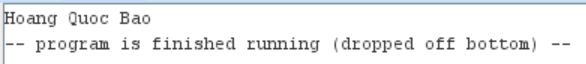
\includegraphics[scale=1]{1}
\end{center}
\pagebreak
\section*{Assignment 2}
\textbf{Mã nguồn: }
\begin{lstlisting}
#Laboratory Exercise 5, Assignment 2
.data
Message1: .asciiz "The sum of ("
Message2: .asciiz ") and ("
Message3: .asciiz ") is ("
Message4: .asciiz ")"
.text
addi $s0, $zero, 0x01341330	# $s0 = 20190000
addi $s1, $zero, 0x1184		# $s1 = 4484
add $s2, $s1, $s0		# $s2 = $s1 + $s0
addi $v0, $zero, 4 		# print string
la $a0, Message1		
syscall

addi $v0, $zero, 1 		# print integer
add $a0, $zero, $s0		# $a0 = $s0
syscall

addi $v0, $zero, 4 		# print string
la $a0, Message2
syscall 

addi $v0, $zero, 1 		# print integer
add $a0, $zero, $s1		# $a0 = $s1
syscall

addi $v0, $zero, 4 		# print string
la $a0, Message3
syscall 

addi $v0, $zero, 1 		# print integer
add $a0, $zero, $s2		# $a0 = $s2
syscall

addi $v0, $zero, 4 		# print string
la $a0, Message4
syscall
\end{lstlisting}
\textbf{Giải thích:}\\
Ta chia chuỗi lớn \colorbox{code}{The sum of (s0) and (s1) is (result)} thành 7 chuỗi nhỏ:
\colorbox{code}{The sum of (} + \colorbox{code}{s0} + \colorbox{code}{) and (} + \colorbox{code}{s1} + \colorbox{code}{) is (} + \colorbox{code}{result} + \colorbox{code}{)}. Chạy từng lệnh syscall để in ra từng chuỗi nhỏ trên.\\
\\\textbf{Kết quả thực hiện: }
\begin{center}
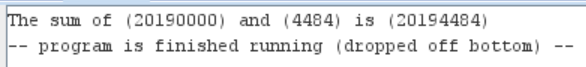
\includegraphics[scale=1]{2}
\end{center}
\pagebreak
\section*{Assignment 3}
\textbf{Mã nguồn:}
\begin{lstlisting}
#Laboratory Exercise 5, Home Assignment 2
.data
x: .space 1000 # destination string x, empty
y: .asciiz "Hoang Quoc Bao\n" # source string y

.text
strcpy:
add $s0,$zero,$zero #s0 = i=0
L1:
la $a1, y	 # $a1 = address of y[0]
la $a0, x	 # $a0 = address of x[0]
add $t1,$s0,$a1 #t1 = s0 + a1 = i + y[0]
lb $t2,0($t1) #t2 = value at t1 = y[i]
add $t3,$s0,$a0 #t3 = s0 + a0 = i + x[0] 
 # = address of x[i]
sb $t2,0($t3) #x[i]= t2 = y[i]
beq $t2,$zero,end_of_strcpy #if y[i]==0, exit
nop
addi $s0,$s0,1 #s0=s0 + 1 <-> i=i+1

j L1 #next character
nop
end_of_strcpy:
# Printf x and y
li $v0, 4
la $a0, x
syscall
la $a0, y
syscall
\end{lstlisting}
\textbf{Giải thích: }\\
Ta duyệt từng phần tử của chuỗi y bằng lệnh \textit{lb} và lưu vào mảng x bằng lệnh \textit{sb}. Chương trình kết thúc khi giá trị y[i] == 0 tức là ta đã duyệt đến cuối mảng.\\
\\\textbf{Kết quả thực hiện:}
\begin{center}
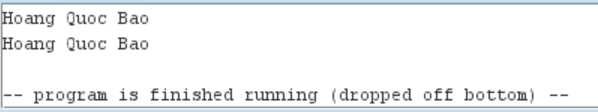
\includegraphics[scale=1]{3}
\end{center}
\pagebreak
\section*{Assignment 4}
\textbf{Mã nguồn:}
\begin{lstlisting}
#Laboratory Exercise 5, Home Assignment 3
.data
string: .space 50
Message1: .asciiz "Nhap xau:"
Message2: .asciiz "Do dai la: "
.text
main:
get_string: 
addi $v0, $zero, 8
la $a0, string
li $a1, 100
syscall
get_length: la $a0, string # a0 = Address(string[0])
 xor $v0, $zero, $zero # v0 = length = 0
 xor $t0, $zero, $zero # t0 = i = 0
check_char: add $t1, $a0, $t0 # t1 = a0 + t0 
 #= Address(string[0]+i) 
 lb $t2, 0($t1) # t2 = string[i]
 beq $t2,$zero,end_of_str # Is null char? 
 addi $v0, $v0, 1 # v0=v0+1->length=length+1
 addi $t0, $t0, 1 # t0=t0+1->i = i + 1
 j check_char
end_of_str: 
end_of_get_length:
print_length:
add $s0, $zero, $v0
addi $v0, $zero, 4
la $a0, Message2
syscall

addi $v0, $zero, 1
add $a0, $s0, $zero
syscall
\end{lstlisting}
\textbf{Giải thích: }\\
Lần lượt duyệt các phần tử trong mảng rồi tăng biến đếm lên 1. Chương trình kết thúc khi string[i] == 0. \textit{(Chú ý: không nên dùng thanh ghi \$v0 để lưu giá trị của biến như trong bài)}
\\\\\textbf{Kết quả thực hiện:}
\begin{center}
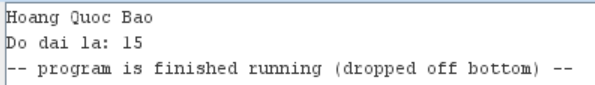
\includegraphics[scale=1]{4}
\end{center}
\pagebreak
\section*{Assignment 5}
\textbf{Mã nguồn:}
\begin{lstlisting}
#Laboratory Exercise 5, Assignment 5
.data
string: .space 100
Message1: .asciiz "Nhap xau: "
Message2: .asciiz "Xau dao nguoc: "
.text
addi $v0, $zero, 4	# printf Message1
la $a0, Message1
syscall

addi $v0, $zero, 8
la $a0, string
li $a1, 20		# set max length = 20
syscall

addi $v0, $zero, 4	# printf Message2
la $a0, Message2
syscall

print_inverse_string:
la $t0, string		# $t0 = string[0]
find_strlen:
add $s1, $t0, $t1	# $t1 = i, $s1 = address of string[i]
lb $s0, 0($s1)		# s0 = string[i]
beq $s0, $zero, traverse_inverse	# branch if i == strlen(string)	
addi $t1, $t1, 1	# i++
j find_strlen

traverse_inverse:
addi $v0, $zero, 11	#print char
print_char:
addi $t1, $t1, -1	# i--
add $s1, $t0, $t1	# s1 = address of string[i]
lb $a0, 0($s1)		# $a0 = string[i]
syscall
beq $t1, $zero, done	# if i == 0 then done
j print_char
done:
\end{lstlisting}
\textbf{Giải thích:}\\
Duyệt mảng theo chiều xuôi để lấy giá trị độ dài của xâu. Sau đó duyệt ngược lại để in ra các chữ theo giá trị đảo ngược.\\\\
\textbf{Kết quả thực hiện:}
\begin{center}
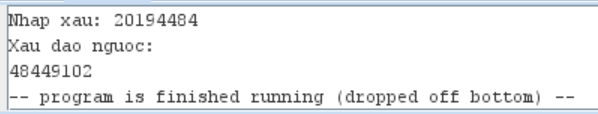
\includegraphics[scale=1]{5}
\end{center}
\end{document}